\documentclass{article}
\usepackage[top=1.1in, bottom=1.5in, left=1in, right=1in]{geometry}
\usepackage{graphicx}
\usepackage[english]{babel}
\usepackage{enumitem}
\usepackage{pdfpages}
\usepackage{tabu}


\begin{document}
\title{Requirements Analysis Document (RAD) for 121Calendar}
\author{Mads Frederik Madsen - mfrm, Holger Stadel Borum - hstb and Paw Høwsgaard Laursen - pawh}
\maketitle
\tableofcontents

%\section{Introduction}
%	\subsection{Purpose of the system}
%	\subsection{Scope of the system}
%	\subsection{Objectives and success citeria the project}
%	\subsection{Definitions, acronyms and abbreveations}
%	\subsection{References}
%	\subsection{Overview}
\section{Current system}
\section{Proposed system}
%	\subsection{Overview}
%	\subsection{Functional Requirements}
	\subsection{Nonfunctional Requirements}
		\subsubsection*{}
		\makebox{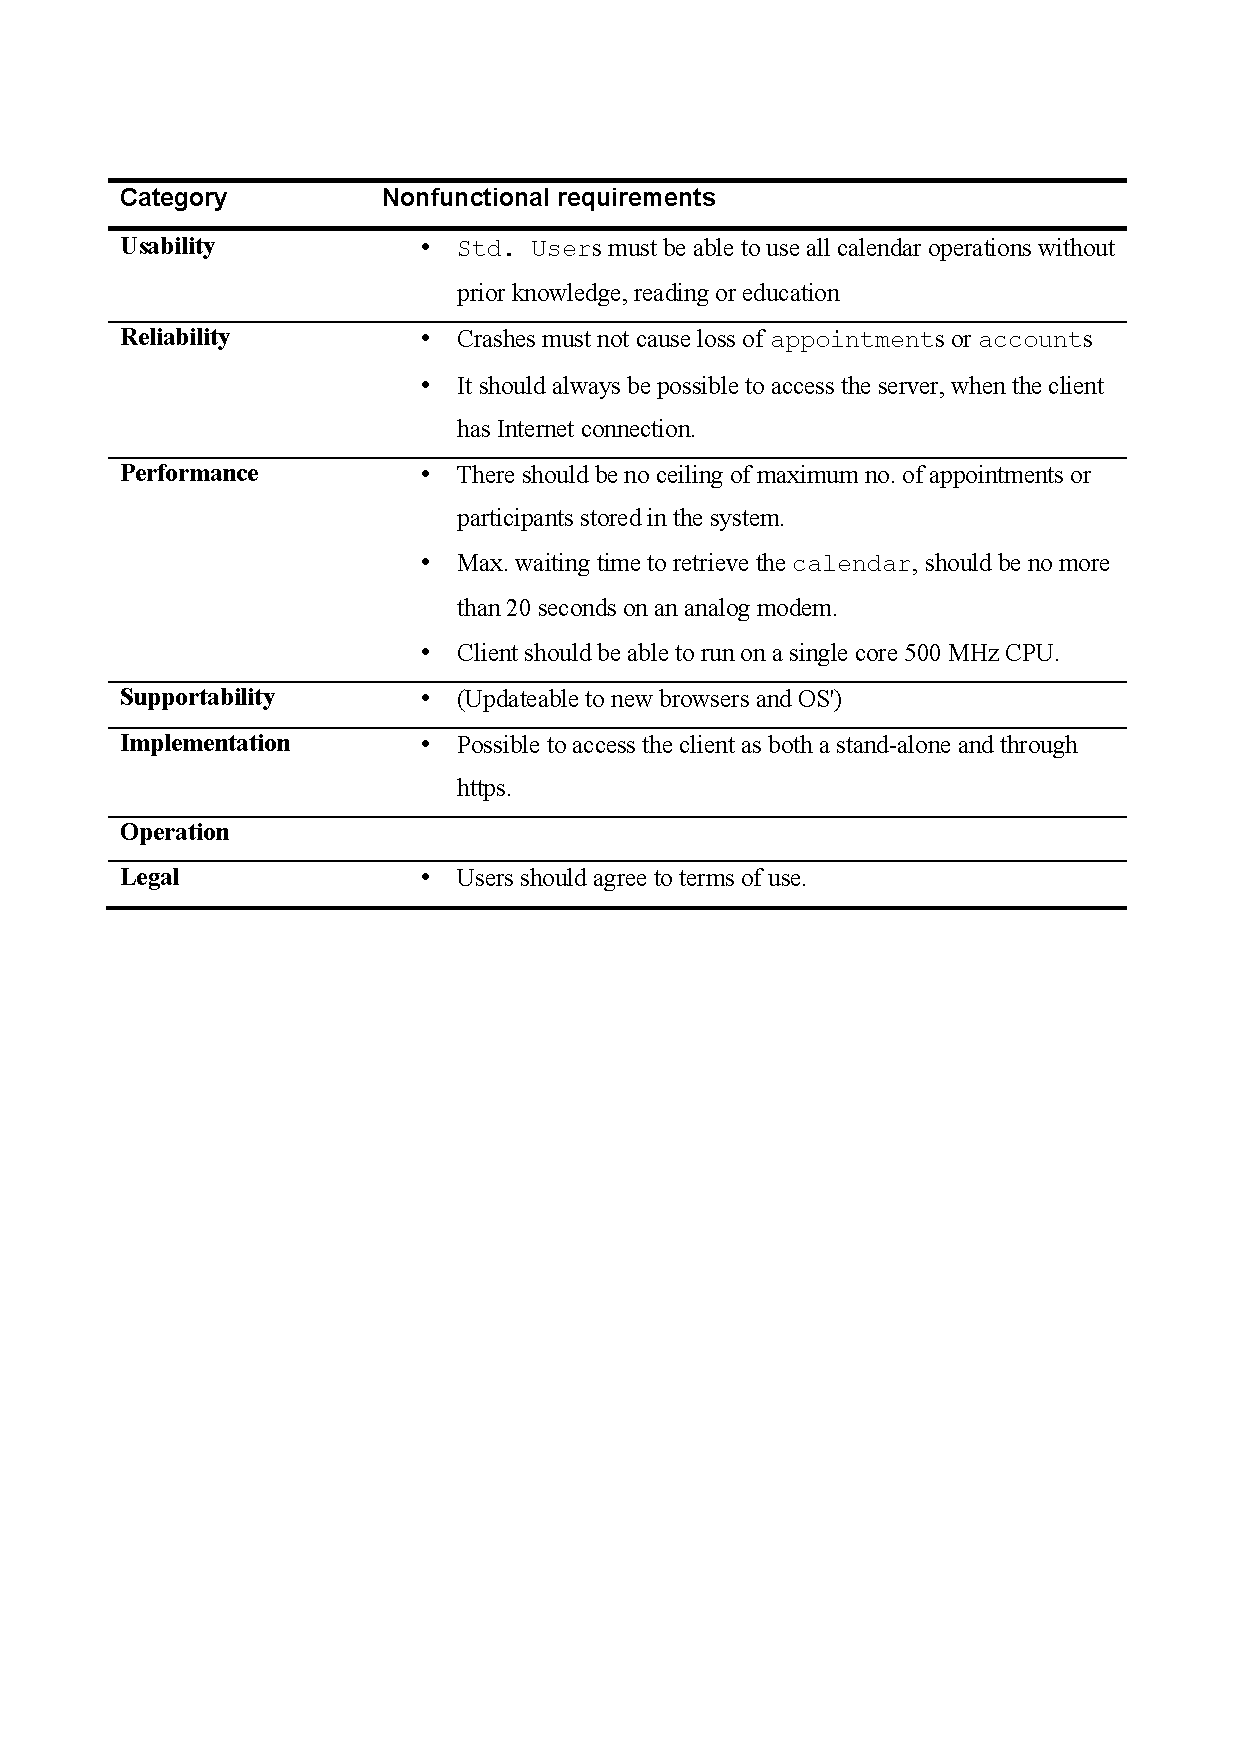
\includegraphics[scale=0.8]{docs/NonfunctionalRequirementsCALENDAR.pdf}}
	\subsection{System models}
		\subsubsection{Scenarios}
			\paragraph{Scenario 1: Create Appointment:}
			 -\\
				\makebox{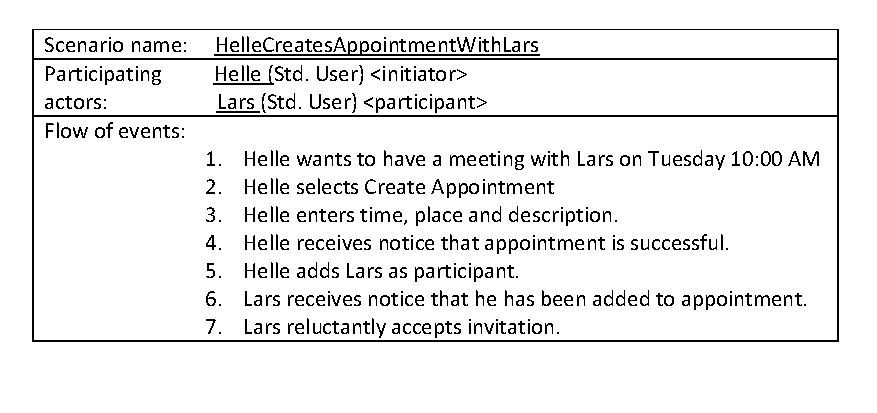
\includegraphics[scale=0.8]{docs/ScCreateApt.pdf}}

			\paragraph{Scenario 2: Create User:}
			 -\\
				\makebox{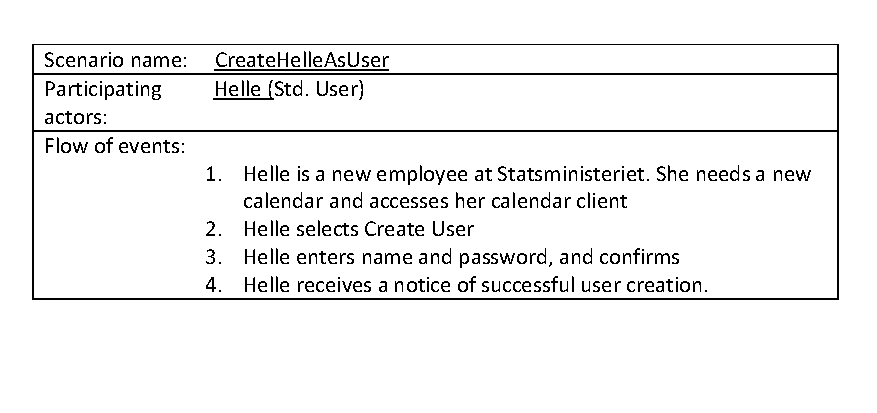
\includegraphics[scale=0.8]{docs/ScCreateUser.pdf}}
			
		\subsubsection{Use case model}
			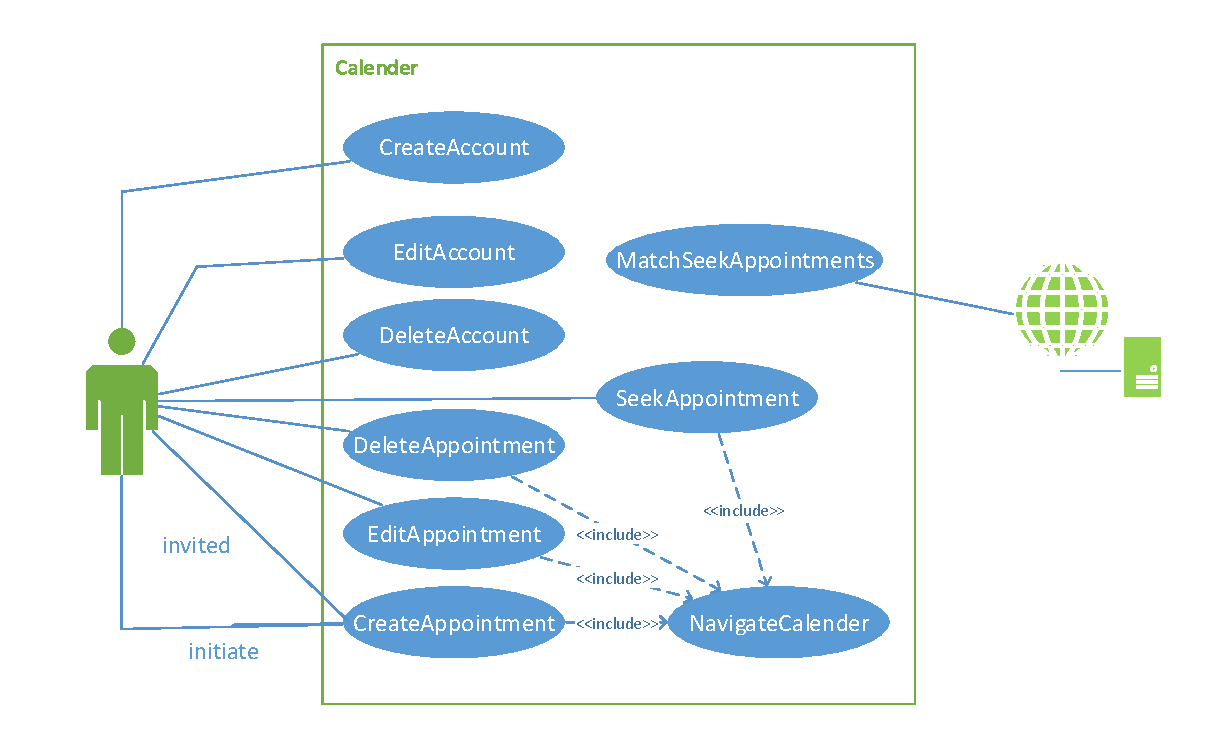
\includepdf{docs/UMLUsecaseDiagramCALENDAR.pdf}
			\begin{center}
				\makebox{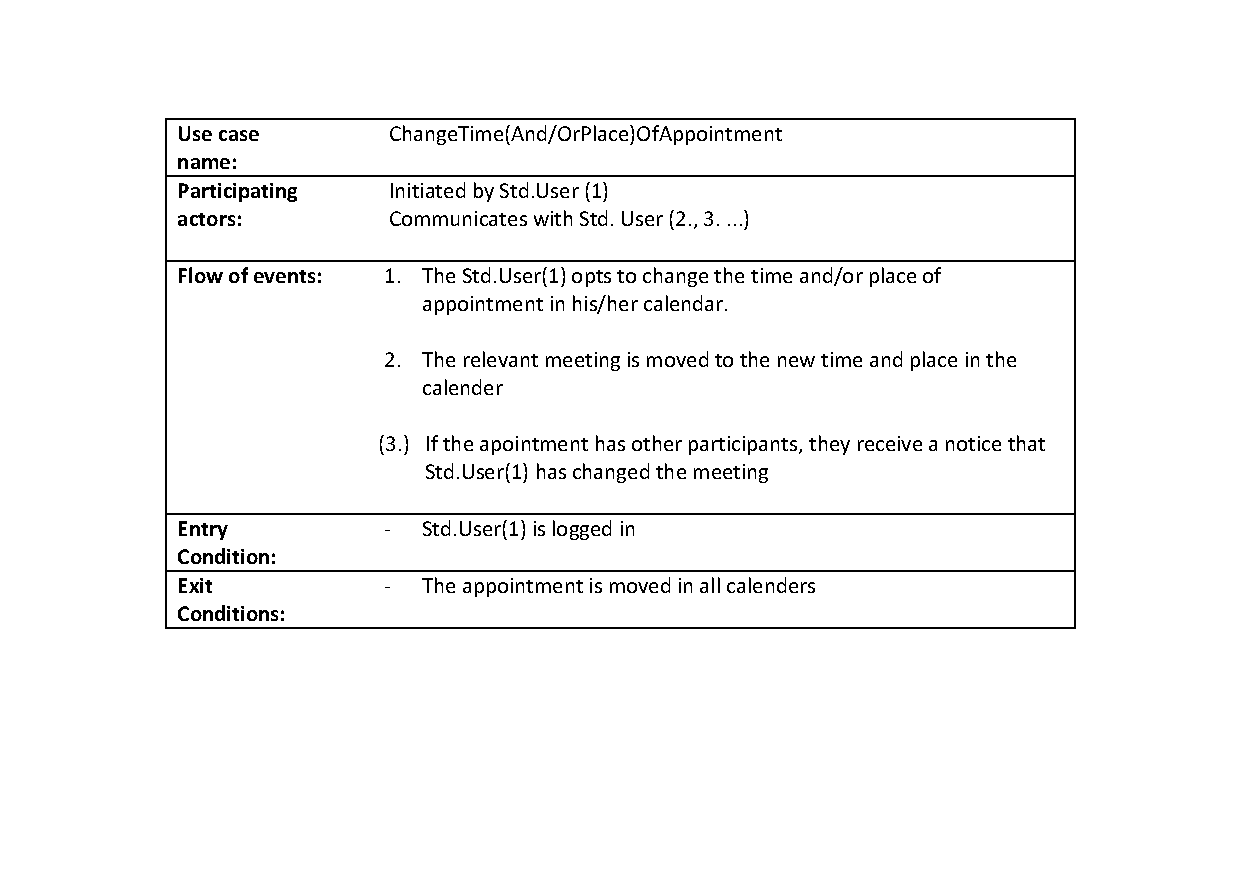
\includegraphics[scale=0.7]{docs/UCChangeTime.pdf}}
				\makebox{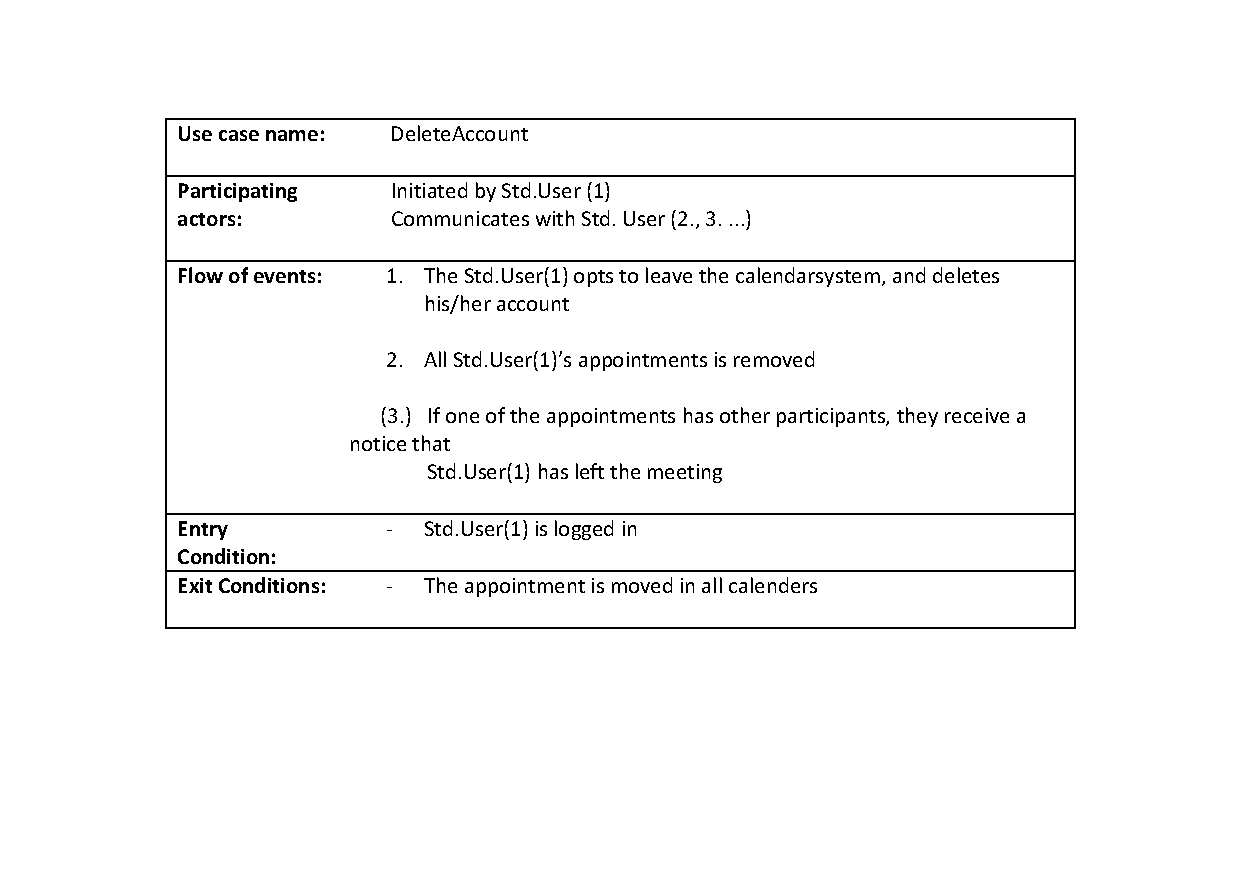
\includegraphics[scale=0.7]{docs/UCDeleteAccount.pdf}}
				\makebox{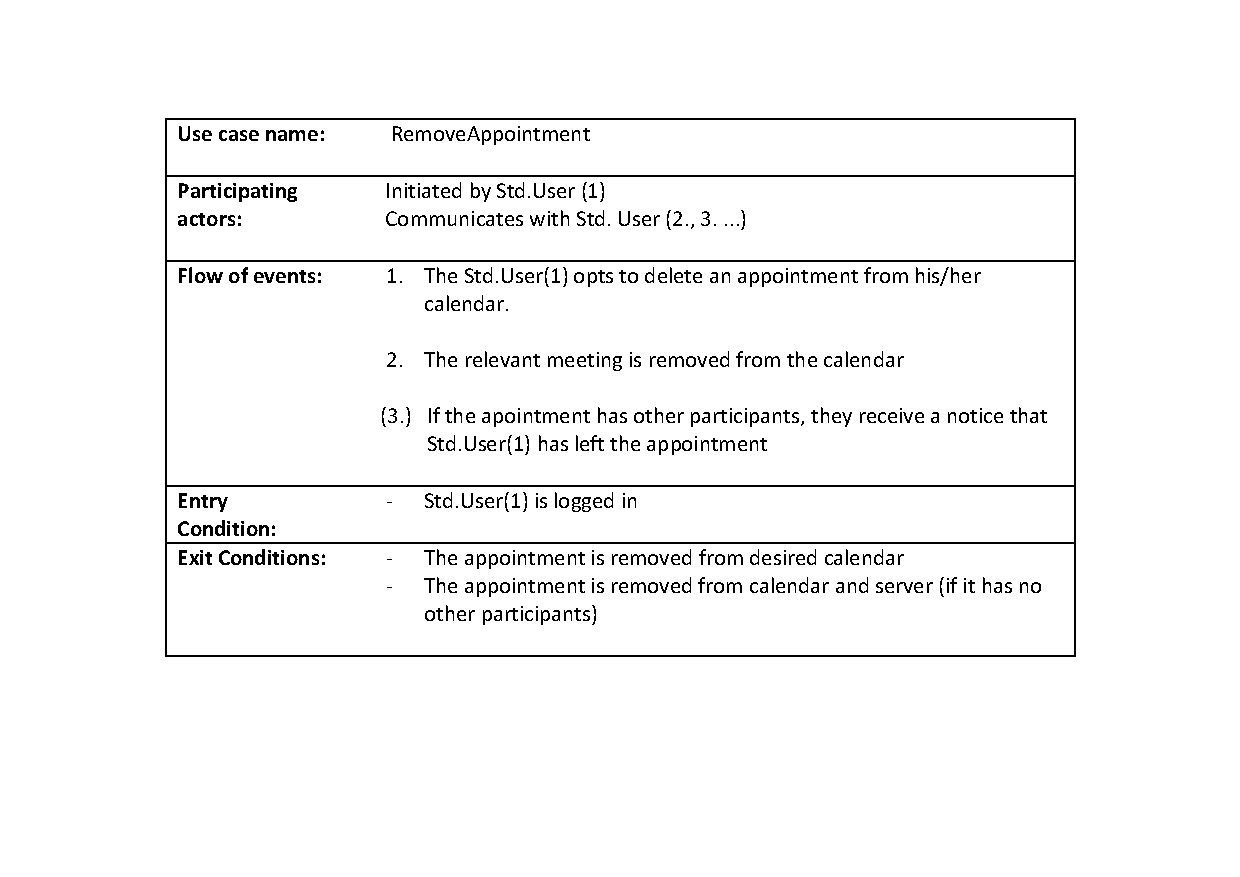
\includegraphics[scale=0.7]{docs/UCRemoveApt.pdf}}
			\end{center}
%		\subsubsection{Object model}
%		\subsubsection{Dynamic model}
%		\subsubsection{User interface}
\section{Glossary}
	\subsection{Initial Analysis Objects:}
	\makebox{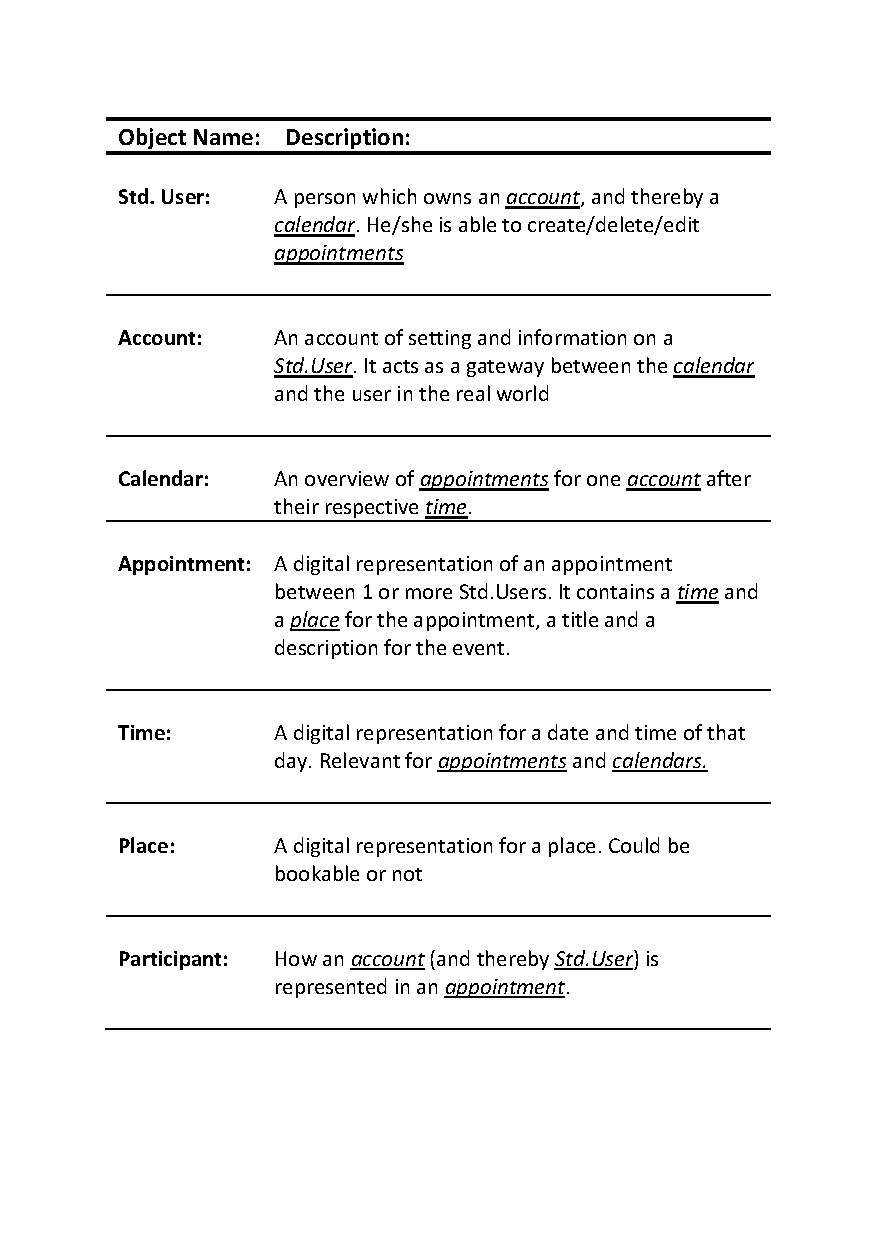
\includegraphics{docs/InitialAnalysisObjects.pdf}}

\end{document}
